\documentclass[12pt, a4paper]{article}

\usepackage[
  margin=1in
]{geometry}

\usepackage[T1, T2A]{fontenc}
\usepackage[utf8]{inputenc}
\usepackage[russian]{babel}
\usepackage{minted}
\usepackage{tabularray}
\usepackage{siunitx}
\usepackage{graphicx}
\usepackage{multicol}

\graphicspath{ {img/} }

\begin{document}

\begin{titlepage}
  \centering
  \textsc{Новосибирский государственный технический университет}\par
  \vspace{1mm}
  Кафедра прикладной математики\par
  \vspace{4cm}
  \textsc{Практическая работа \textnumero 6}\par
  {\huge\bfseries Параллельные алгоритмы на графах\par}
  \vspace{1cm}
  {\scriptsize ФПМИ, ПМ-24\par}
  \vspace{1mm}
  {\itshape\large Параскун И., Шакиров П., Герасименко В.\par}
  \vfill
  {\small преподаватель\par}
  \vspace{1mm}
  \textsc{Домников Петр Александрович}
  \vfill
  \large{Новосибирск, 2024}
\end{titlepage}


\setcounter{page}{2}
\tableofcontents

\newpage

\section{Постановка задачи}
Изучить и реализовать параллельный алгоритм Дейкстры для поиска кратчайших путей между всеми парами вершин графа.
Провести тестирование разработанных подпрограмм.

\begin{itemize}
  \item Граф хранится в виде списков смежности;
  \item Результат работы программы - матрица кратчайших путей;
  \item Инструмент параллельных вычислений - OpenMP.
\end{itemize}

\section{Текст программы}

\inputminted[firstline=6, lastline=26]{c}{/home/mehandes/c/src/github.com/paraskun/math/bgs/dcg/include/bgs/dcg.h}
\inputminted[firstline=11]{c}{/home/mehandes/c/src/github.com/paraskun/math/bgs/dcg/src/dcg.c}

\section{Тестирование}
\subsection{Проверка работоспособности}
Работоспособность программы проверялась на следующем графе:

\vspace{5mm}
\begin{center}
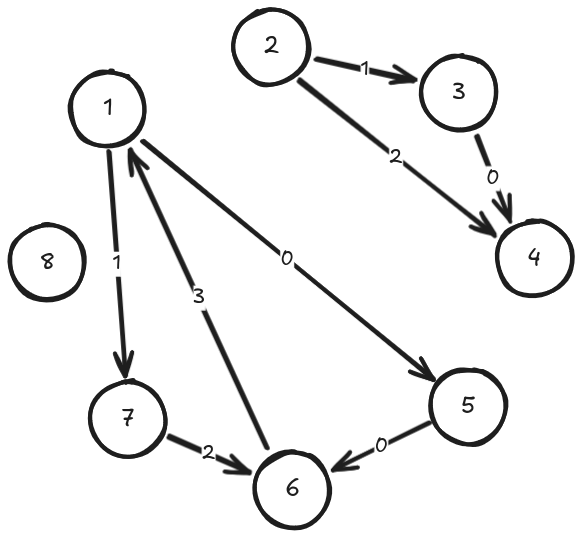
\includegraphics[scale=0.3]{./img/1.png}
\end{center}
\vspace{5mm}

\noindentгде справа изображён результирующий граф. Результат работы программы в текстовом виде приведен ниже.

\begin{minted}{console}
1 -> 1 [0.000000]: 1 - 1
1 -> 5 [0.000000]: 1 - 5
1 -> 6 [0.000000]: 1 - 5 - 6
1 -> 7 [1.000000]: 1 - 7
2 -> 2 [0.000000]: 2 - 2
2 -> 3 [1.000000]: 2 - 3
2 -> 4 [1.000000]: 2 - 3 - 4
3 -> 3 [0.000000]: 3 - 3
3 -> 4 [0.000000]: 3 - 4
4 -> 4 [0.000000]: 4 - 4
5 -> 1 [3.000000]: 5 - 6 - 1
5 -> 5 [0.000000]: 5 - 5
5 -> 6 [0.000000]: 5 - 6
5 -> 7 [4.000000]: 5 - 1 - 7
6 -> 1 [3.000000]: 6 - 1
6 -> 5 [3.000000]: 6 - 1 - 5
6 -> 6 [0.000000]: 6 - 6
6 -> 7 [4.000000]: 6 - 1 - 7
7 -> 1 [5.000000]: 7 - 6 - 1
7 -> 5 [5.000000]: 7 - 1 - 5
7 -> 6 [2.000000]: 7 - 6
7 -> 7 [0.000000]: 7 - 7
8 -> 8 [0.000000]: 8 - 8
\end{minted}

\subsection{Оценка производительности}

\begin{table}[H]
\centering
\begin{tblr}{
  width=\textwidth, 
  colspec={|c|X|X|X|X|X|},
  rowspec={|c|c|c|c|}
}
\SetCell[r=2]{c} $N$  & \SetCell[c=5]{c} Time, s                                                      \\
                      & \SetCell{c} 1 & \SetCell{c} 2 & \SetCell{c} 4 & \SetCell{c} 8 & \SetCell{c} 12  \\
1E+03                 & 0.08972276    & 0.04521948    & 0.03510834    & 0.02947188    & 0.02425874      \\
1E+04                 & 8.83093987    & 4.50553548    & 2.31318906    & 1.64102111    & 1.22599482
\end{tblr}
\caption{Время выполнения подпрограммы для графов различной размерности.}
\end{table}

\begin{table}[H]
\centering
\begin{tblr}{
  width=\textwidth, 
  colspec={|c|X|X|X|X|X|},
  rowspec={|c|c|c|c|}
}
\SetCell[r=2]{c} $N$  & \SetCell[c=5]{c} Acceleration                                                   \\
                      & \SetCell{c} 1 & \SetCell{c} 2 & \SetCell{c} 4 & \SetCell{c} 8 & \SetCell{c} 12  \\
1E+03                 & 1.00000000    & 1.98416169    & 2.55559676    & 3.04435143    & 3.69857462      \\
1E+04                 & 1.00000000    & 1.96002005    & 3.81764726    & 5.38136884    & 7.20308090
\end{tblr}
\caption{Ускорение подпрограммы для графов различной размерности.}
\end{table}

\newpage

\section{Вывод}

\begin{center}
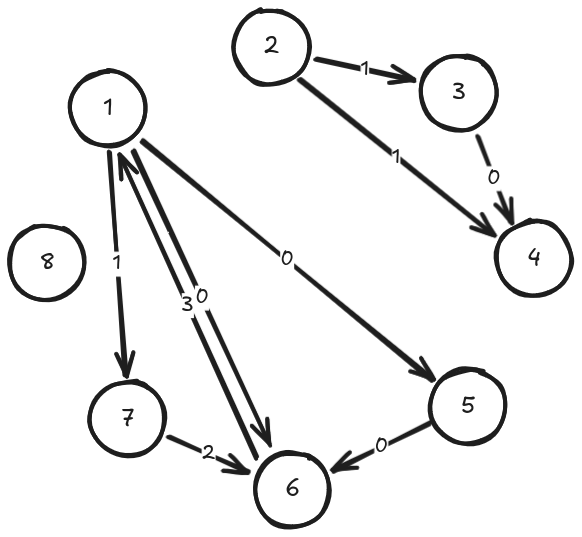
\includegraphics[scale=0.7]{./img/2.png} \\
\vspace{6mm}
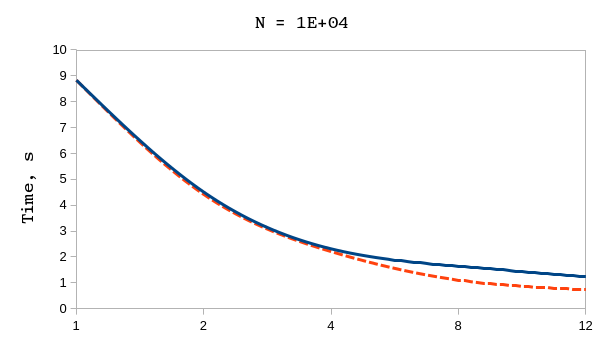
\includegraphics[scale=0.7]{./img/3.png}
\end{center}
\vspace{6mm}

Оценивая полученные результаты, можно сделать вывод, что параллельный алгоритм Дейкстры для поиска кратчайших
путей между всеми парами вершин графа обладает свойством линейного ускорения.

\newpage

\section{Вспомогательные структуры данных}
\subsection{Связный список}
\inputminted[firstline=6]{c}{/home/mehandes/c/src/github.com/paraskun/math/dsa/src/sll/psll.c}

\subsection{Очередь по приоритетам}
\inputminted[firstline=8]{c}{/home/mehandes/c/src/github.com/paraskun/math/dsa/src/pque/ppque.c}

\subsection{Хеш-множество}
\inputminted[firstline=8]{c}{/home/mehandes/c/src/github.com/paraskun/math/dsa/src/hset/uhset.c}

\end{document}

